
% VLDB template version of 2020-08-03 enhances the ACM template, version 1.7.0:
% https://www.acm.org/publications/proceedings-template
% The ACM Latex guide provides further information about the ACM template

\documentclass[sigconf, nonacm]{acmart}

%% The following content must be adapted for the final version
% paper-specific
%\newcommand\vldbdoi{XX.XX/XXX.XX}
%\newcommand\vldbpages{XXX-XXX}
% issue-specific
%\newcommand\vldbvolume{14}
%\newcommand\vldbissue{1}
%\newcommand\vldbyear{2020}
% should be fine as it is
%\newcommand\vldbauthors{\authors}
%\newcommand\vldbtitle{\shorttitle} 
% leave empty if no availability url should be set
%\newcommand\vldbavailabilityurl{URL_TO_YOUR_ARTIFACTS}
% whether page numbers should be shown or not, use 'plain' for review versions, 'empty' for camera ready
%\newcommand\vldbpagestyle{plain} 

\begin{document}
\title{Home Loan Default Prediction with Machine Learning}

%%
%% The "author" command and its associated commands are used to define the authors and their affiliations.
\author{Sakib Sadman Shajib}
\affiliation{%
  \institution{North South University}
  \department{Department of Electrical and Computer Engineering}
}
\email{sakib.shajib173@northsouth.edu}

\author{Ilmiat Farhana}
\affiliation{%
  \institution{North South University}
  \department{Department of Electrical and Computer Engineering}
}
\email{ilmia.farhana@northsouth.edu}

\author{Tahmid Hasan Nafi}
\affiliation{%
  \institution{North South University}
  \department{Department of Electrical and Computer Engineering}
}
\email{tahmid.nafi@northsouth.edu}

\author{Iftekhar Alam Pial}
\affiliation{%
  \institution{North South University}
  \department{Department of Electrical and Computer Engineering}
}
\email{iftekhar.pial@northsouth.edu}

%%
%% The abstract is a short summary of the work to be presented in the
%% article.
\begin{abstract}
Prediction of loan repayment ability is an active area of research. Several machine learning models exist that explore this in great detail. In this paper, we explore the effect of feature engineering with a combination of several models, and compare their ability to classify an applicant as risky or safe, in their ability to repay a loan.

{\bf Keywords:}machine learning, classification, loan default risk, feature engineering.

\end{abstract}

\maketitle

%%% do not modify the following VLDB block %%
%%% VLDB block start %%%
%\pagestyle{\vldbpagestyle}
%\begingroup\small\noindent\raggedright\textbf{PVLDB Reference Format:}\\
%\vldbauthors. \vldbtitle. PVLDB, \vldbvolume(\vldbissue): \vldbpages, \vldbyear.\\
%\href{https://doi.org/\vldbdoi}{doi:\vldbdoi}
%\endgroup
%\begingroup
%\renewcommand\thefootnote{}\footnote{\noindent
%This work is licensed under the Creative Commons BY-NC-ND 4.0 International License. Visit %\url{https://creativecommons.org/licenses/by-nc-nd/4.0/} to view a copy of this license. For any use %beyond those covered by this license, obtain permission by emailing %\href{mailto:info@vldb.org}{info@vldb.org}. Copyright is held by the owner/author(s). Publication rights %licensed to the VLDB Endowment. \\
%\raggedright Proceedings of the VLDB Endowment, Vol. \vldbvolume, No. \vldbissue\ %
%ISSN 2150-8097. \\
%\href{https://doi.org/\vldbdoi}{doi:\vldbdoi} \\
%}\addtocounter{footnote}{-1}\endgroup
%%% VLDB block end %%%

%%% do not modify the following VLDB block %%
%%% VLDB block start %%%
%\ifdefempty{\vldbavailabilityurl}{}{
%\vspace{.3cm}
%\begingroup\small\noindent\raggedright\textbf{PVLDB Artifact Availability:}\\
%The source code, data, and/or other artifacts have been made available at \url{\vldbavailabilityurl}.
%\endgroup
%}
%%% VLDB block end %%%

\section{Introduction}

Over the past decades, home credit default risk has been an important topic for discussion, as many people struggle to get loans for houses, on grounds of having an insufficient or incomplete credit history. In some cases, the applicant may have no credit history whatsoever. Banks are usually hasty to hand out loans to such applicants, and commonly they are discriminated against. Given that a notable portion of the US neighborhoods consists of people belonging to different cultures, ethnic minorities, and color, there is good reason for a Bank to have an evaluation for the risk of handing out a house loan to an applicant. Making better decisions may lead to cheaper loans in the long run, and reduce discrimination, and improve quality of life for the immigrants/applicants with insufficient credit histories. Our paper aims to use domain knowledge feature engineering in combination with standard classification algorithms to obtain a predictive model, and compare their performance.

\section{Immediate Problem}
Analyzing default-ability of Home Loan Lenders using Machine Learning Models

\section{Methodology}
Research location and data collection, Data Observation and Data Pre-processing.

\subsection{Research location and data collection}

In this study, the credit defaulting data collected from the United States only. The source of data\cite{dataset} is Home Credit - A financial institution that hands out loans to applicants with an incomplete credit history. The main dataset is split into training and testing. Both contain 122 columns of data that contain fields such as annual income, number of children, gender, number of days of employment at their workplace, age in days etcetera. There are a few supporting datasets such as bureau data, credit card data, previous application and their installment payments, Point of Sales transactions.

\subsection{Data Observation}
The training data is unbalanced, in that a significantly higher proportion of people in our sample are able to repay loans compared to people who default on loans, as reflected by the histogram: 

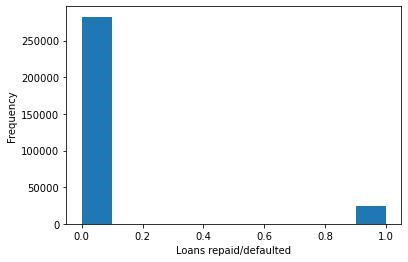
\includegraphics[width=\linewidth]{figures/fig.jpg}

For each of the 122 features, we calculated the correlation coefficient with the target value, and we observed that the age of the participant yields the strongest positive correlation, of 0.0782, since the value of age is negative in our datasets, but true in absolute value, we obtain that the younger an applicant is, the less likely he is to be able to repay the loan. We observe the following distribution of age in our data:  

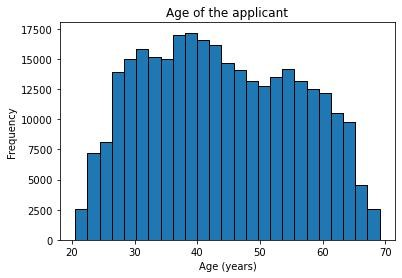
\includegraphics[width=\linewidth]{figures/FIG2.jpg}

When we plot the age of the population with their corresponding loan repay ability values (orange indicates that loans are not repaid) in a Kernel Density Estimate plot, we observe an interesting trend

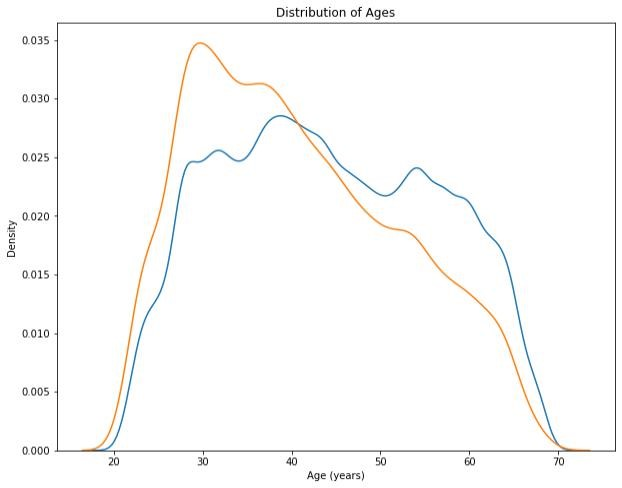
\includegraphics[width=\linewidth]{figures/FIG3.jpg}

From the figure above we can make a few interesting observations, namely that the distribution of the defaulters have a positive skew, and have a peak towards the left side. Which, points out that, in general it is much riskier to lend to the younger population compared to the older population.

However, as for the negative correlation coefficients, we obtain significantly stronger values of correlation for EXT SOURCE 3,2 and 1; the coefficients being -0.179, -0.160, and -0.155 respectively. EXT SOURCE in our data indicates data from external undisclosed sources, but the documentation states that it is a metric identical to credit rating. Thus it makes sense that the higher a credit rating is for someone, the less likely he is to default on a loan repayment.

\subsection{Data Pre-Processing}

We have First pre-process the data. We have used two types of pre-processing here. One is label encoding and the other is one hot encoding.

\subsubsection{Label Encoding}

We have used label encoding for two unique features and removed gender with invalid input, invalid days from phone number changed and created a categorical age feature.

\subsubsection{One Hot Encoding}

We have used one hot encoding for the rest of the datasets. The categorical data is processed with one hot encoder.

\subsection{Feature engineering}

Using domain knowledge, we aggregated several features to include the relationship between certain features we believe to be useful for our model. The features we introduced, in order of decreasing importance, is

\subsubsection{CREDIT TO ANNUITY RATIO}

This feature encodes the relationship between the credit and annuity of an applicant; trial and error suggest this to be the most important feature, with the greatest normalized importance rating.

\subsubsection{EXT SOURCES MEAN}

EXT SOURCE in our data indicates a credit score of the applicant from a third party undisclosed source, and it would seem that the mean credit score across all sources play a huge role in determining the risk of loan defaulting.

\subsubsection{CREDIT TO GOODS RATIO}

This encodes the credit of an applicant to the price of the good for which the loan is given

\subsubsection{EXT SOURCES MIN}

This is one of the over-fitted features which was derived from External Sources.

\subsubsection{GROUP CREDIT TO ANNUITY MEAN}

This an aggregate feature encoding the credit of an applicant to the mean amount of his loan annuity.

We had 1200 features to work it.

\subsection{Algorithms}

In combination with feature engineering, the following models were used:

\subsubsection{Logistic Regression}

Logistic Regression is a binary classifier; It is a mathematical model that uses a logistic function to model the output. Because the underlying model is actually linear regression, logistic regression works well when the data are linearly separable.

We can train a logistic regression model in different ways. One common way is to minimize the cross-entropy loss function through an iterative process. i.e:

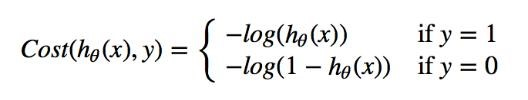
\includegraphics[width=\linewidth]{figures/EQN1.jpg}

Where we Minimize J( ) by Gradient Descent, altering :

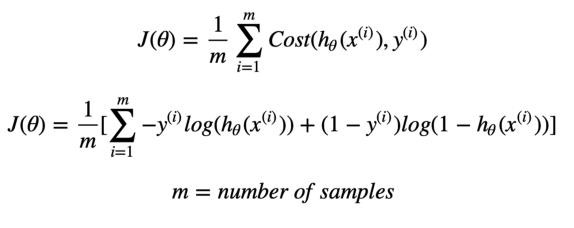
\includegraphics[width=\linewidth]{figures/EQN2.jpg}

\subsubsection{Random Forest}

Random Forest is an ensemble method, the predictor is a group of independent decision trees, for training the decision trees, it picks random subsets of features and tries to search for the most important feature from the subset by splitting nodes. Usually this is accompanied by using random weights/thresholds for each feature, as done in an ordinary decision tree. Classification is achieved by outputting the mode of all of the independent decision trees.

\subsubsection{XGBoost}

XGBoost\cite{xgb} was first proposed by Chen et al. as an implementation of a GBM(Gradient Boosting Machines); it is widely regarded as one of the best performing algorithms for supervised learning. It makes predictions through an ensemble tree method of K independent decision trees, i.e:

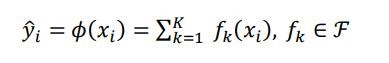
\includegraphics[width=\linewidth]{figures/EQN3.jpg}

The objective of XGBoost is to find the optimal set of functions f k that minimize the sum of the loss function and the regularization objective (shown below), using Gradient Tree Boosting. It does this iteratively for each step t by using second order approximations.

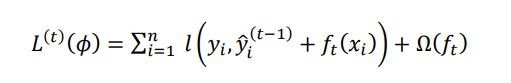
\includegraphics[width=\linewidth]{figures/EQN4.jpg}

\subsubsection{LightGBM}

Also an implementation of a GBM(Gradient Boosting Machine), LightGBM\cite{lightgbm} is functionally the same as XGBoost, the only structural difference between the two is observed when a node is split. While XGBoost uses a pre-sorted algorithm in combination with a linear scan to find the optimal set of features in a subsample, LightGBM uses a novel technique, called GOSS(Gradient-based One-Side Sampling)\cite{goss}, based on randomized sampling techniques, and is therefore, significantly faster than XGBoost.

\section{Evaluation and Metrics}

We use the following metrics to compare the performance of different models:

\subsection{Area under ROC}
An ROC/receiver operating characteristic curve is a graphical representation of the ability of a Binary Classifier to identify a class correctly or not. It is created by plotting the true positive rate (sensitivity/recall) of the binary classifier, against the false positive rate. We use the area under the ROC curve as a metric of how well a model performs.
A random classifier will have an expected area under ROC of 0.5, whereas a perfect classifier that is 100percent correct will have an area under ROC of 1. and a perfectly incorrect classifier, that is incorrect 100 percent of the time, will have an ROC of 0.

\begin{figure}[htp]
    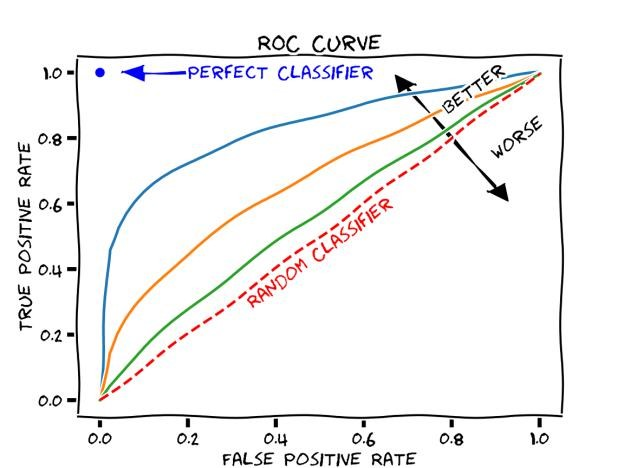
\includegraphics[width=\linewidth]{figures/EQN5.jpg}
    \caption{A pictorial representation of the area under ROC curve\cite{xkcd}}
\end{figure}

\section{Result and Decision}
We found that GBTree performed the best with the engineered features compared to any other model. The area under ROC metric for all the models tested are shown below:

\begin{tabular}{|c|c|c|c|c|}
\hline
    Score & Logistic & Random & LightGBM & XGBoost \\
        & Regression & Forest & & \\
\hline
    Public & 0.73962 & 0.73139 & 0.79480 & 0.76661 \\
    Private & 0.73723 & 0.72396 & 0.79228 & 0.76317 \\
\hline
\end{tabular}


%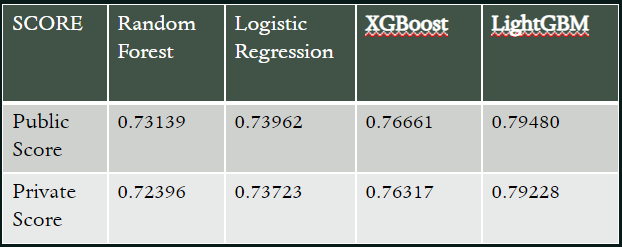
\includegraphics[width=\linewidth]{figures/final result.PNG}

We observe that LightGBM outperformed the other models in its diagnostic ability to classify risk; We also observe that XGBoost without feature engineering performs particularly well, comparable to Logistic Regression, and Random Forest methods with features engineered.

We also see that XGBoost performs similarly to LightGBM, this was to be expected given that they both share the same underlying mechanics sans node splitting methodology. It is to be noted that XGBoost takes significantly longer, and takes up more memory than LightGBM.

\section{Possible Improvement}

Since LightGBM has shown promising results even using almost default settings, we'll try to tweak the model and see if anything performs. From experiments, we have found that GBM algorithms work much better for structured data like the current dataset. We will look into other implementation of GBM as well.

Another possible improvement over our current method that we have not explored, would be to have a hybrid model of a Neural Network and a Gradient Boosting Machine in combination with a framework for hyperparameter optimization. We have found the perfect model for that DeepGBM\cite{deepgbm}. We will explore this in the future.

\begin{acks}
 The completion of this paper would not have been possible without the continuous support and enlightenment provided by our faculty, Dr. Nabeel Mohammed, Assistant Professor, North South University.
\end{acks}

%\clearpage

\begin{thebibliography}{99}
\bibliographystyle{ACM-Reference-Format}
\bibitem{dataset} Home Credit Default Risk, Kaggle

\bibitem{xgb}	T. Chen and C. Guestrin, “XGBoost: a scalable tree boosting system,” in Proc. ACM SIGKDD International Conference on Knowledge Discovery & Data Mining, pp. 785-794, 2016

\bibitem{xkcd}	Xkcd comics: A pictorial representation of the area under ROC curve https://commons.wikimedia.org/wiki/File:Roc-draft-xkcd-style.svg
\bibitem{lightgbm}	Guolin Ke et al, “LightGBM: A Highly Efficient Gradient Boosting Decision Tree” in Conference on Neural Information Processing Systems 2017


\bibitem{gbmbench}Andreea Anghel, Nikolaos Papandreou, Thomas Parnell, Alessandro De Palma, Haralampos Pozidis (2019) Benchmarking and Optimization of Gradient Boosting Decision Tree
Algorithms arXiv arXiv:1809.04559 .

\bibitem{deepgbm} Guolin Ke,Zhenhui Xu, Jia Zhang, Jiang Bian, Tie-Yan Liu. KDD '19: Proceedings of the 25th ACM SIGKDD International Conference on Knowledge Discovery & Data MiningJuly 2019

\bibitem{discussionlightgbm} Abdelwahed Assklou and Aguiar. \href{https://www.kaggle.com/c/home-credit-default-risk/discussion/64580}{7th solution - **Not great things but small things in a great way.**}. {\em Kaggle}.

\bibitem{lgbm:2017} Guolin Ke, Qi Meng, Thomas Finley, Taifeng Wang, Wei Chen, Weidong Ma, Qiwei Ye, Tie-Yan Liu (2017). LightGBM: A Highly Efficient Gradient Boosting Decision Tree. {\em Academia.edu}.


\bibitem{goss} Andreea Anghel, Nikolaos Papandreou, Thomas Parnell, Alessandro De Palma, Haralampos Pozidis (2019). Benchmarking and Optimization of Gradient Boosting Decision Tree Algorithms. {\em arXiv} 	arXiv:1809.04559 .



\end{thebibliography}

%\bibliographystyle{ACM-Reference-Format}
%\bibliography{sample}

\end{document}
\endinput
